\documentclass{../shipyard-slide}

\usepackage[british]{babel}
\usepackage[british]{datetime2}
\usepackage{amsmath}
\usepackage{amssymb}
\usepackage{ulem}
\usepackage{qrcode}
\usepackage{wasysym}

\usepackage{tikz,calc}
\usetikzlibrary{shapes, shapes, arrows, chains, fit, quotes}

\tikzstyle{trienode} = [draw=text-color, rounded corners]
\tikzstyle{bucket} = [draw=text-color, rectangle]

\settheme{ipfs-camp-2022}

%Information to be included in the title page:
\title{DHT Interoperability}
\subtitle{Bridging Networks through Kademlia}
\author{Gui Michel}
\avatar{../resources/avatar.jpg}
\handle{@guissou}
\group{Probelab}
\institute{Interplanetary Shipyard}
\event{IPFS Camp}
\date{\DTMdate{2024-07-12}}

\begin{document}

\frame{\titlepage}

\logo{
	\vspace{7cm}
	
\includegraphics[scale=.1]{../shipyard-resources/ipfs-camp-logo.png}
	\hspace{4em}
}

\begin{frame}
\frametitle{Kademlia DHT}

\begin{columns}[onlytextwidth]
	\begin{column}{0.64\textwidth}
		\begin{itemize}
			\itemc A Distributed Hash Table (DHT) is a decentralized overlay network used for peer and content routing
			\itemc Nodes identified by a binary \texttt{Key}, determining nodes location in the Keyspace
			\itemc Highly scalable
			\begin{itemize}
				\item[\greencube] State: $\log{N}$
				\item[\greencube] Lookup: $\log{N}$
			\end{itemize}
			\itemc Routing table stores nodes into \textit{buckets} based on their distance from the local node's \texttt{Key}
		\end{itemize}
	\end{column}
		\begin{column}{0.34\textwidth}
    		\begin{center}
        		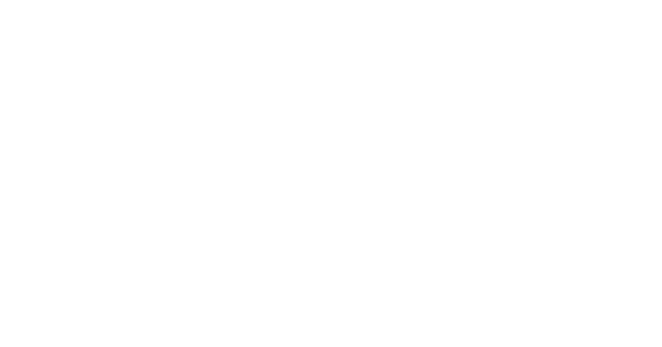
\includegraphics[width=13em]{resources/kademlia-trie.png}
        		\textit{Kademlia Binary Trie}
    		\end{center}
	\end{column}

\end{columns}
\end{frame}

\begin{frame}
\frametitle{Kademlia: Keyspace \& Routing Table}

\hspace{4cm}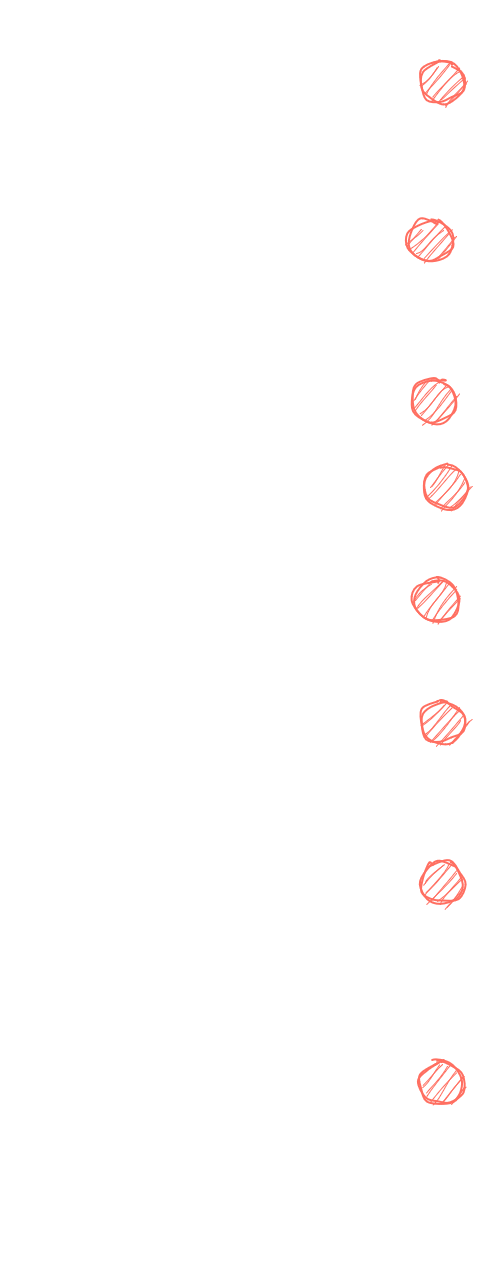
\includegraphics[scale=.13]{resources/rt0-0.png}
\end{frame}

\begin{frame}
\frametitle{Kademlia: Keyspace \& Routing Table}

\hspace{4cm}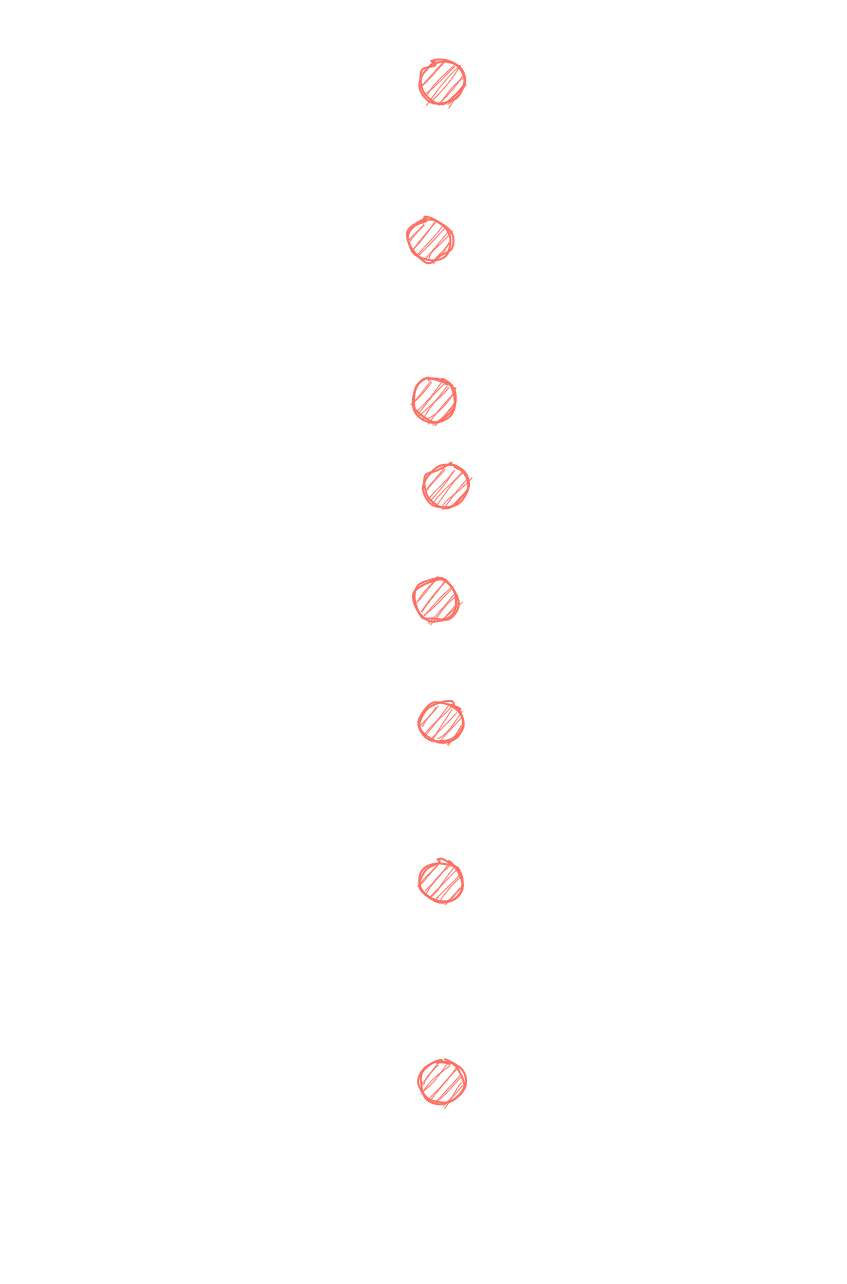
\includegraphics[scale=.13]{resources/rt0-1.png}
\end{frame}


\begin{frame}
\frametitle{Kademlia: Keyspace \& Routing Table}

\hspace{4cm}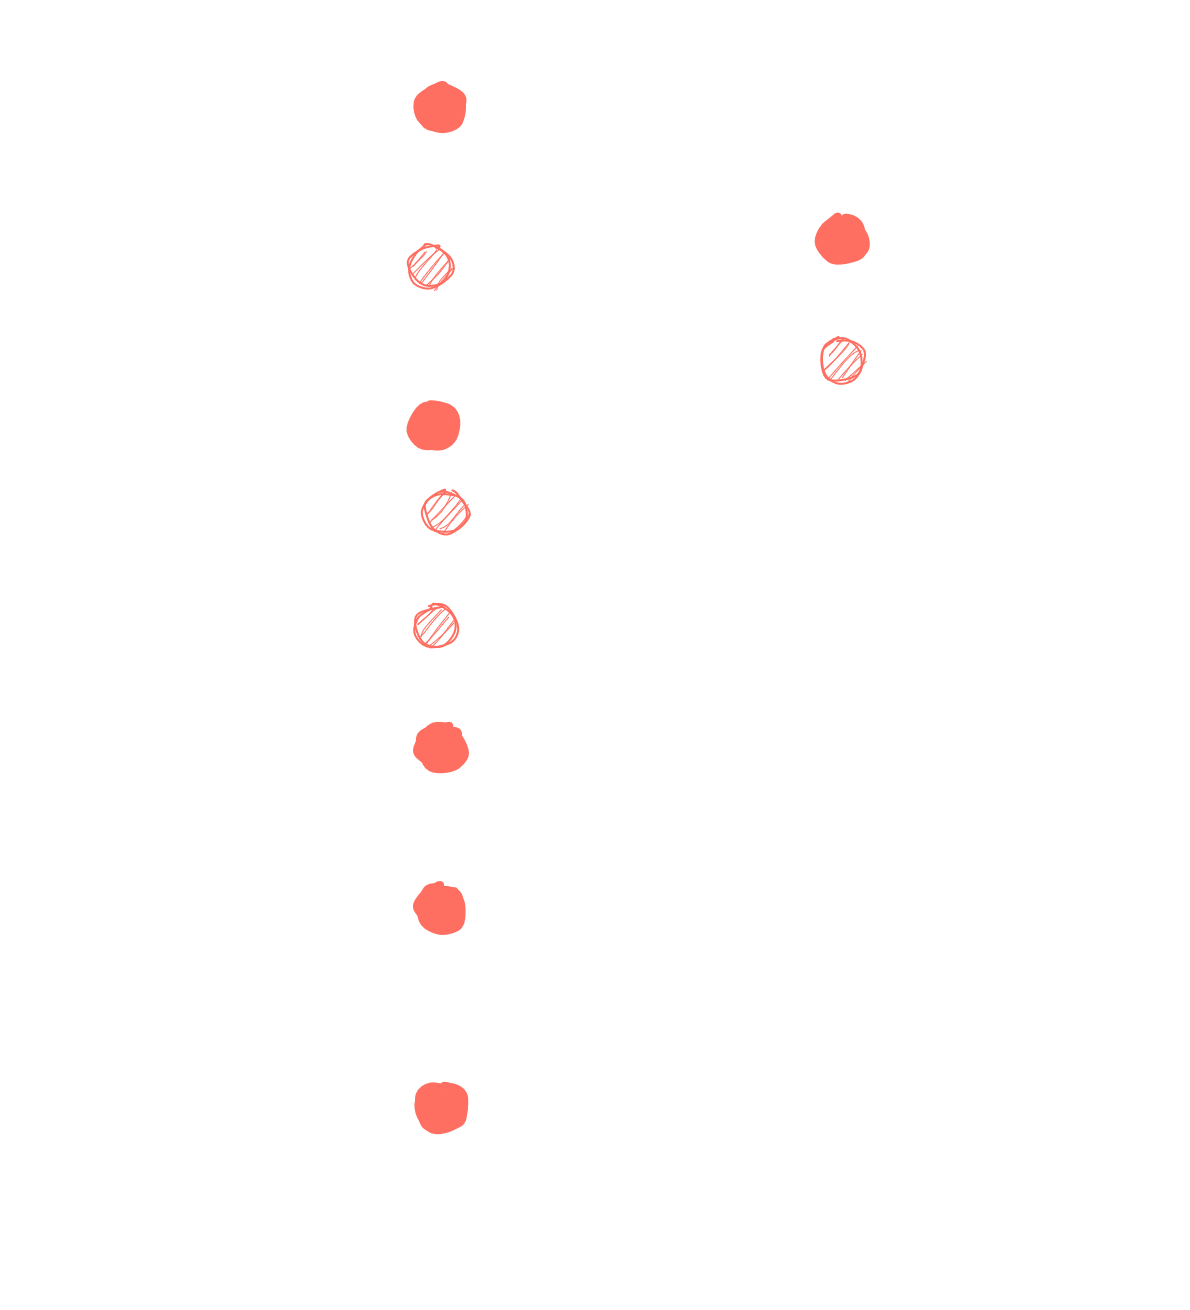
\includegraphics[scale=.13]{resources/rt0-2.png}
\end{frame}


\begin{frame}
\frametitle{Routing Table Maintainance}

\begin{itemize}
	\itemc Routing Table state is $\mathcal{O}(\log{N})$ with $N$ being the network size.
	\itemc State in memory is small
	\itemc Maintenance can be expensive
	\begin{itemize}
		\item[\greencube] Unresponsive peers should be removed from the table $\Rightarrow$ all peers stored in the routing table must be periodically probed
		\item[\greencube] Nodes must periodically lookup their own identity to be aware of their closest neighbors\\
		\item[\greencube] Larger routing table $\Rightarrow$ higher network load
	\end{itemize}
\end{itemize}
\end{frame}

\begin{frame}
\frametitle{DHT disambiguation}

\begin{itemize}
	\itemc DHT Protocol $\xrightarrow{}$ \texttt{libp2p kad-dht}, \texttt{ethereum discovery}
	\itemc DHT Implementation $\xrightarrow{}$ \texttt{go-libp2p-kad-dht}, \texttt{@libp2p/kad-dht}
	\itemc DHT Swarm $\xrightarrow{}$ \texttt{Amino DHT}, \texttt{Filecoin DHT}
\end{itemize}
\end{frame}


\begin{frame}
\frametitle{What is DHT interop and why we want it?}

\begin{itemize}
	\itemc Participation in multiple DHT swarms
	\itemc Protocol evolution
	\itemc Transports compatibility
	\itemc Improved network security
	\itemc Network bootstrapping
\end{itemize}

\end{frame}

\begin{frame}
\frametitle{What we DON'T want to do}

\begin{itemize}
	\itemc Merge existing DHTs
	\itemc One DHT to rule them all
	\itemc Impose a global standard for all DHTs
\end{itemize}
\end{frame}

\begin{frame}
\frametitle{Layers within DHT implementations}

\begin{enumerate}
	\item Wire format
	\item Transport
	\item Encryption
	\item Identity
	\item Kademlia
\end{enumerate}
\end{frame}

\begin{frame}
\frametitle{Using two DHT networks}

\begin{itemize}
	\itemc Assume we build a client \texttt{Hexo} to retrieve content from IPFS in the Amino DHT and from Bittorrent Mainline DHT \smiley
	\itemc \texttt{Hexo} needs to participate in both Kademlia DHTs
	\itemc State is double, maintenance is $2x$ more expensive \frownie
	\itemc Many open connections \frownie
\end{itemize}

\vspace{1cm}

{\Large \;}

\end{frame}

\begin{frame}
\frametitle{Using two DHT networks}

\begin{itemize}
	\itemc Assume we build a client \texttt{Hexo} to retrieve content from IPFS in the Amino DHT and from Bittorrent Mainline DHT \smiley
	\itemc \texttt{Hexo} needs to participate in both Kademlia DHTs
	\itemc State is double, maintenance is $2x$ more expensive \frownie
	\itemc Many open connections \frownie
\end{itemize}

\vspace{1cm}

{\Large This can be optimized!}

\end{frame}

\begin{frame}
\frametitle{Example: Amino-Mainline Bridge}
\end{frame}


\begin{frame}
\frametitle{Example: Amino-Mainline Bridge}

\hspace{2cm}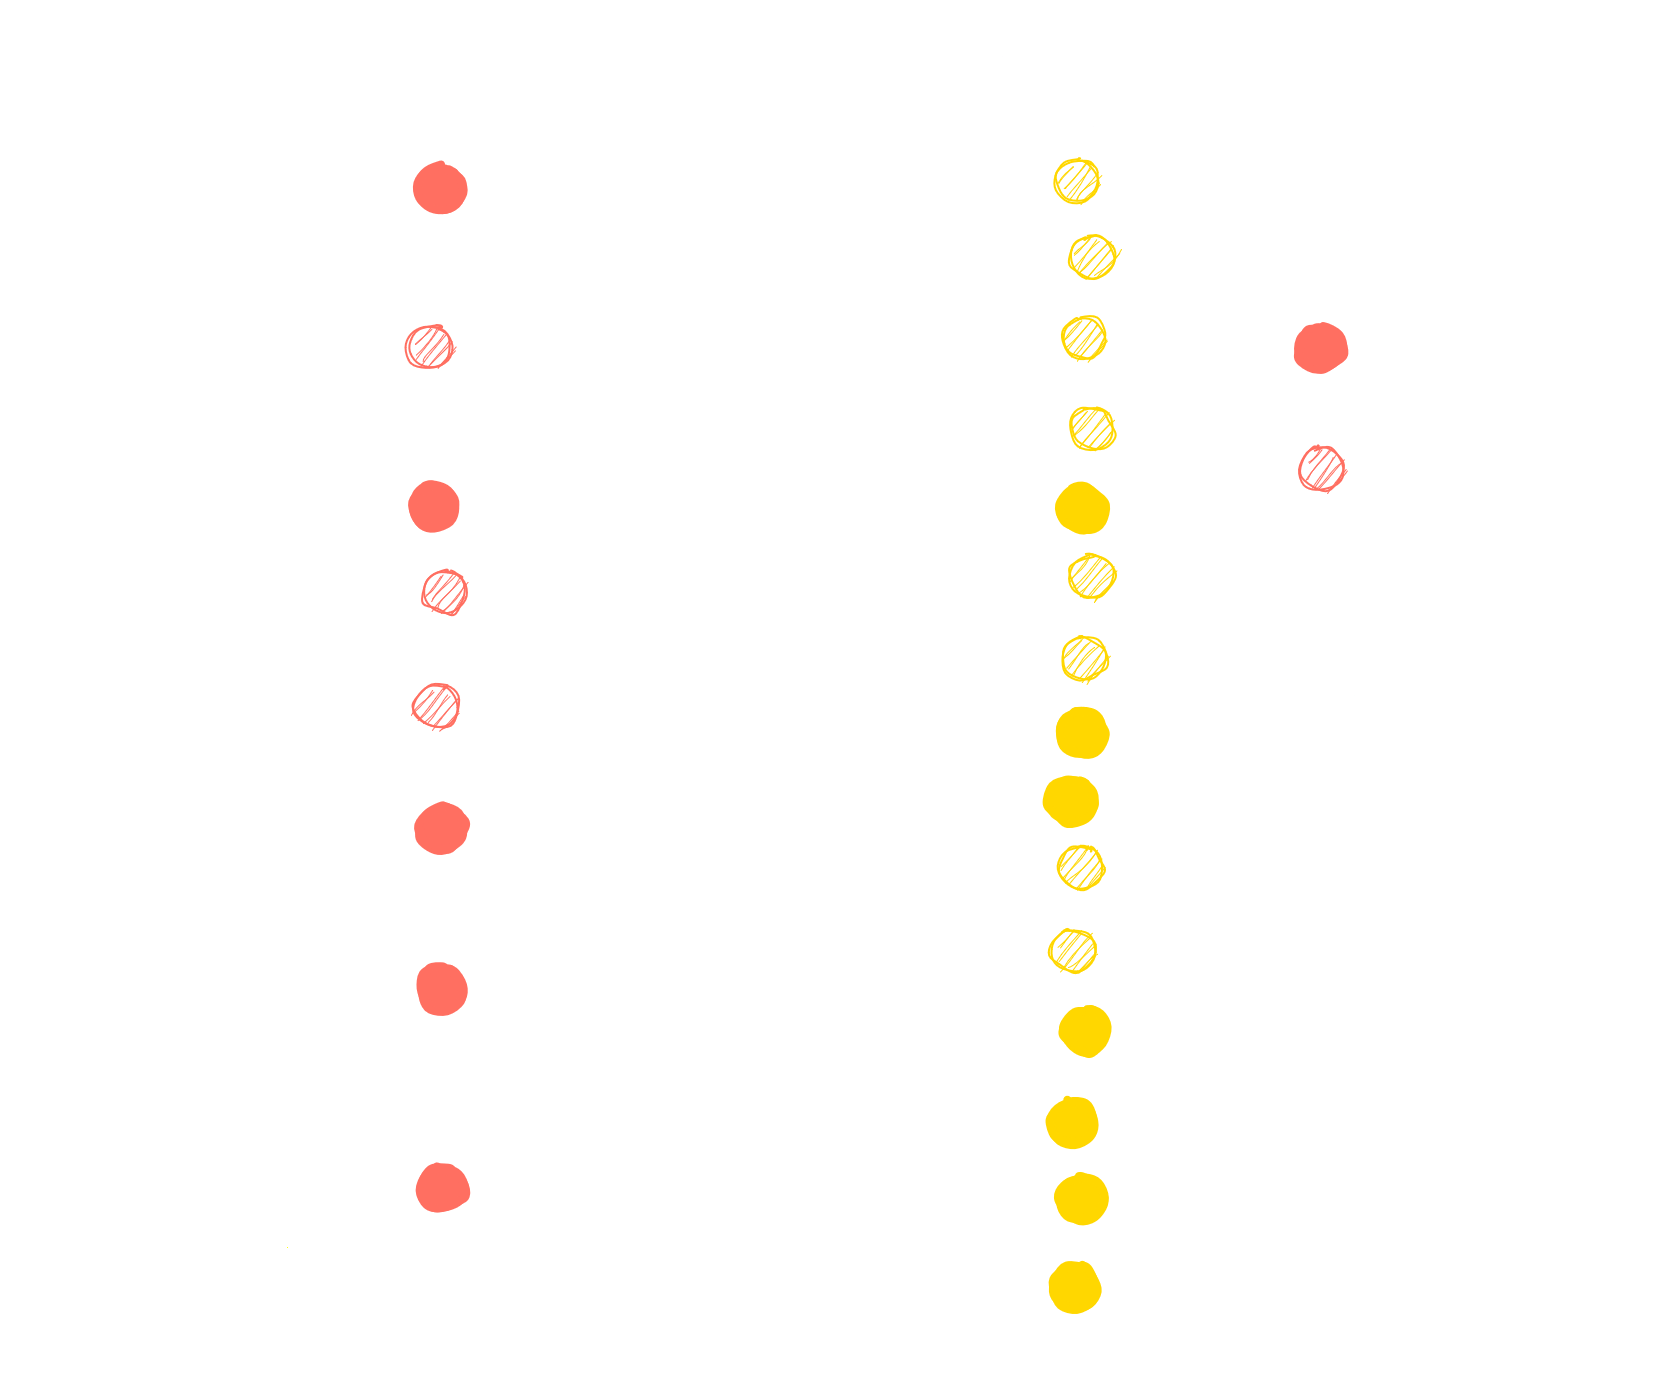
\includegraphics[scale=.13]{resources/rt1-0.png}
\end{frame}

\begin{frame}
\frametitle{Example: Amino-Mainline Bridge}

\hspace{2cm}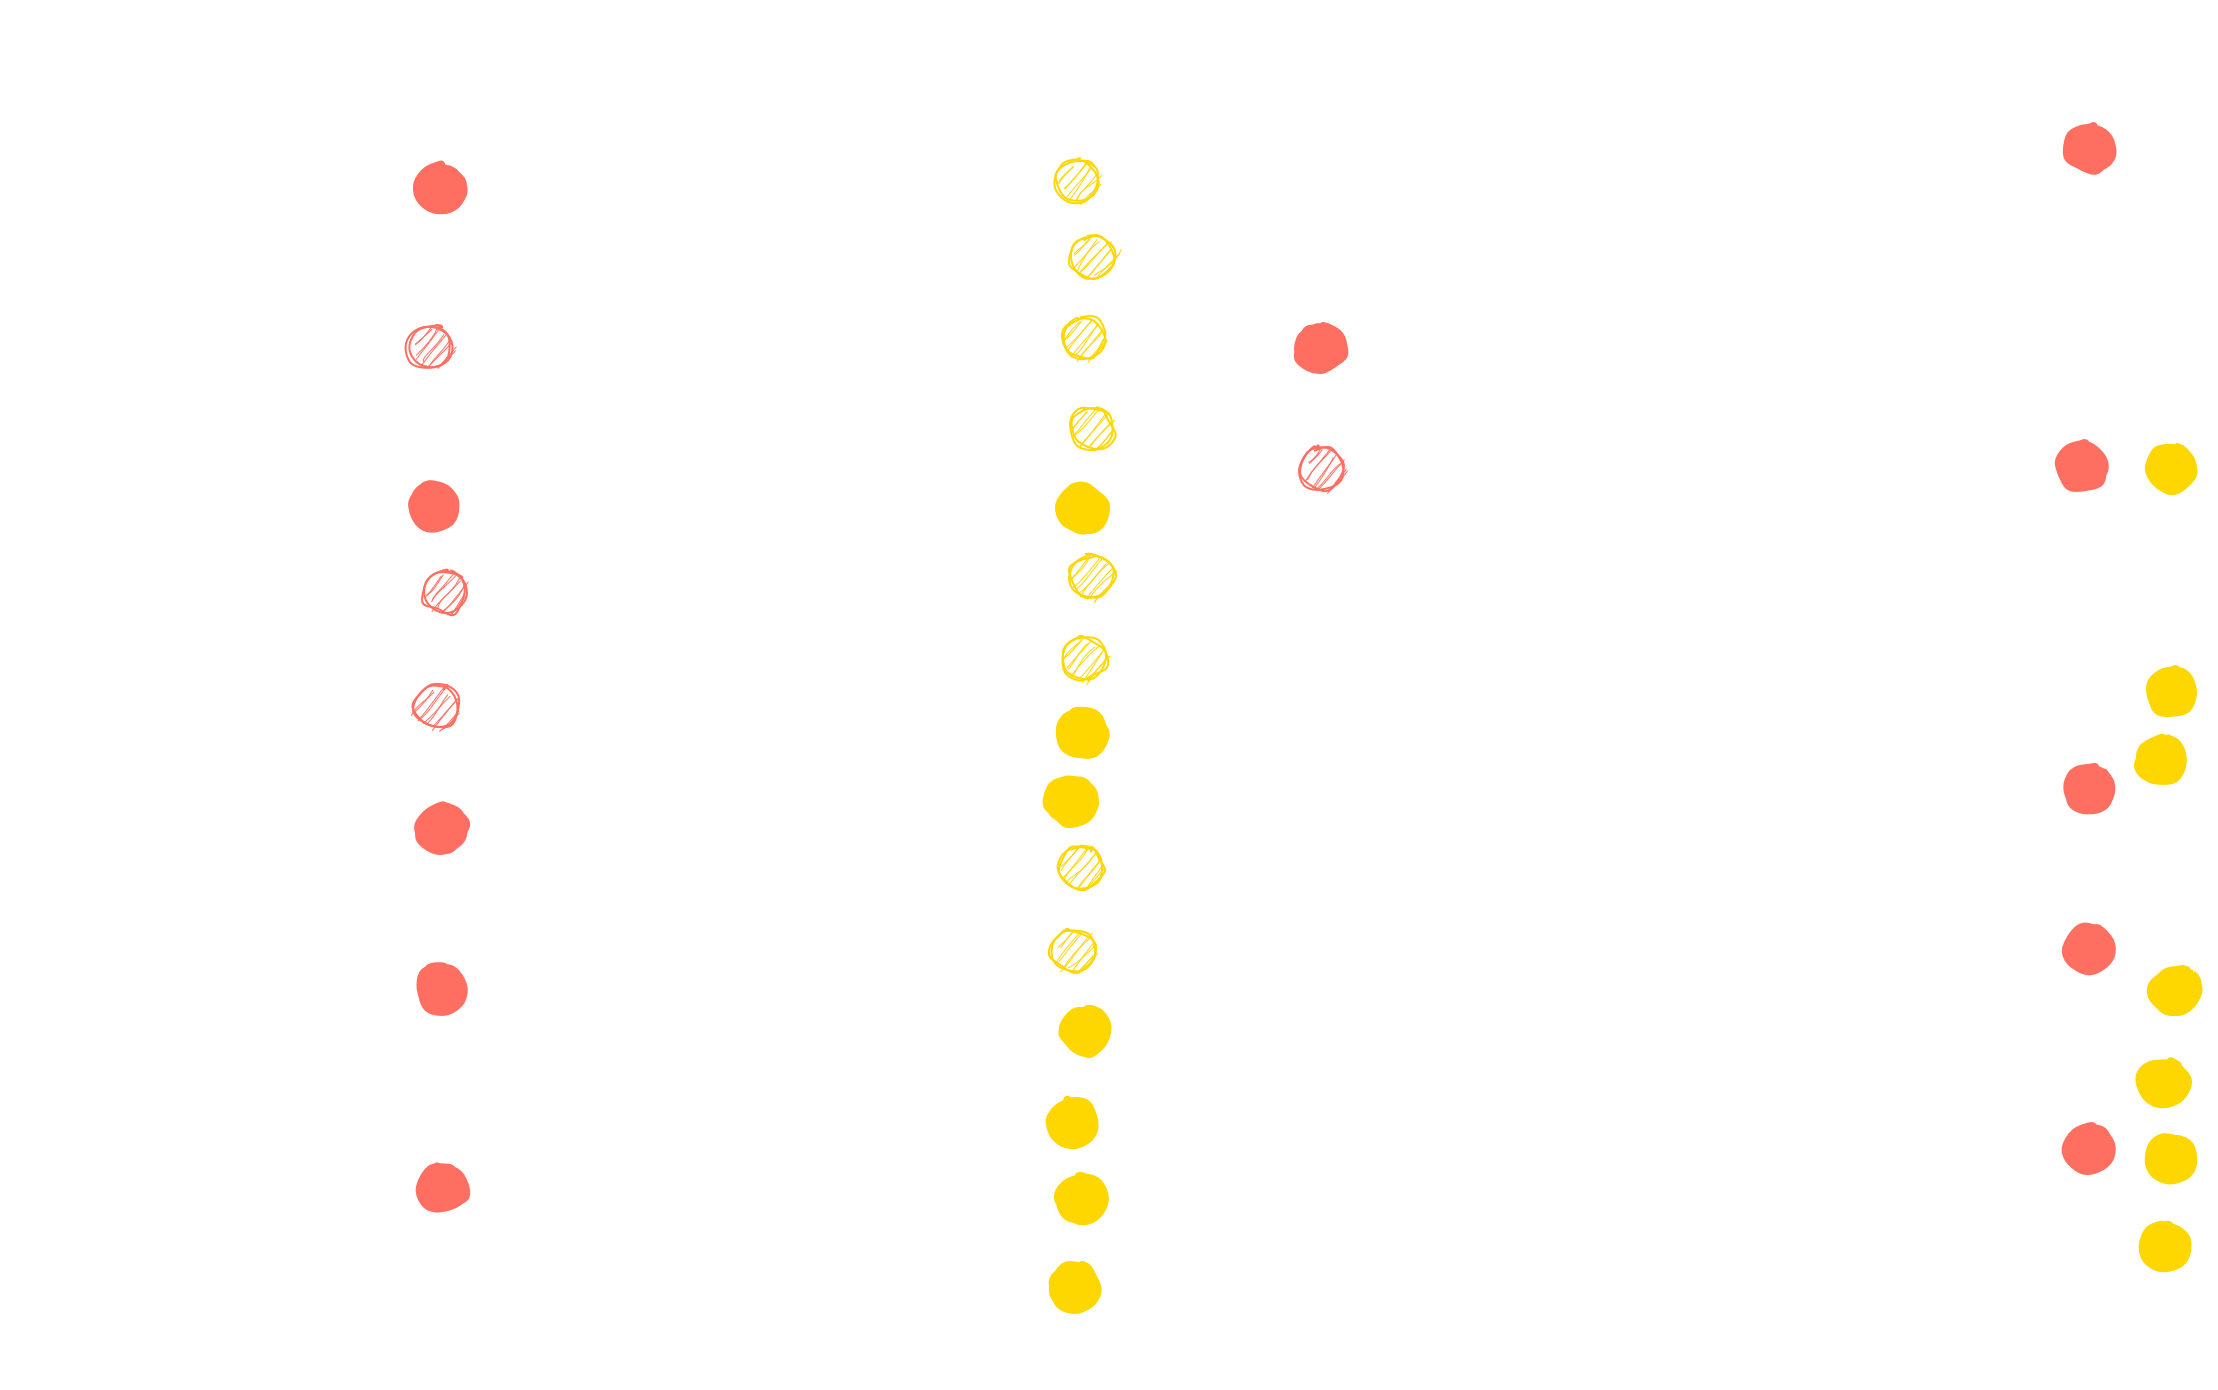
\includegraphics[scale=.13]{resources/rt1-1.png}

\end{frame}

\begin{frame}
\frametitle{Example: Amino-Mainline Bridge}

\hspace{2cm}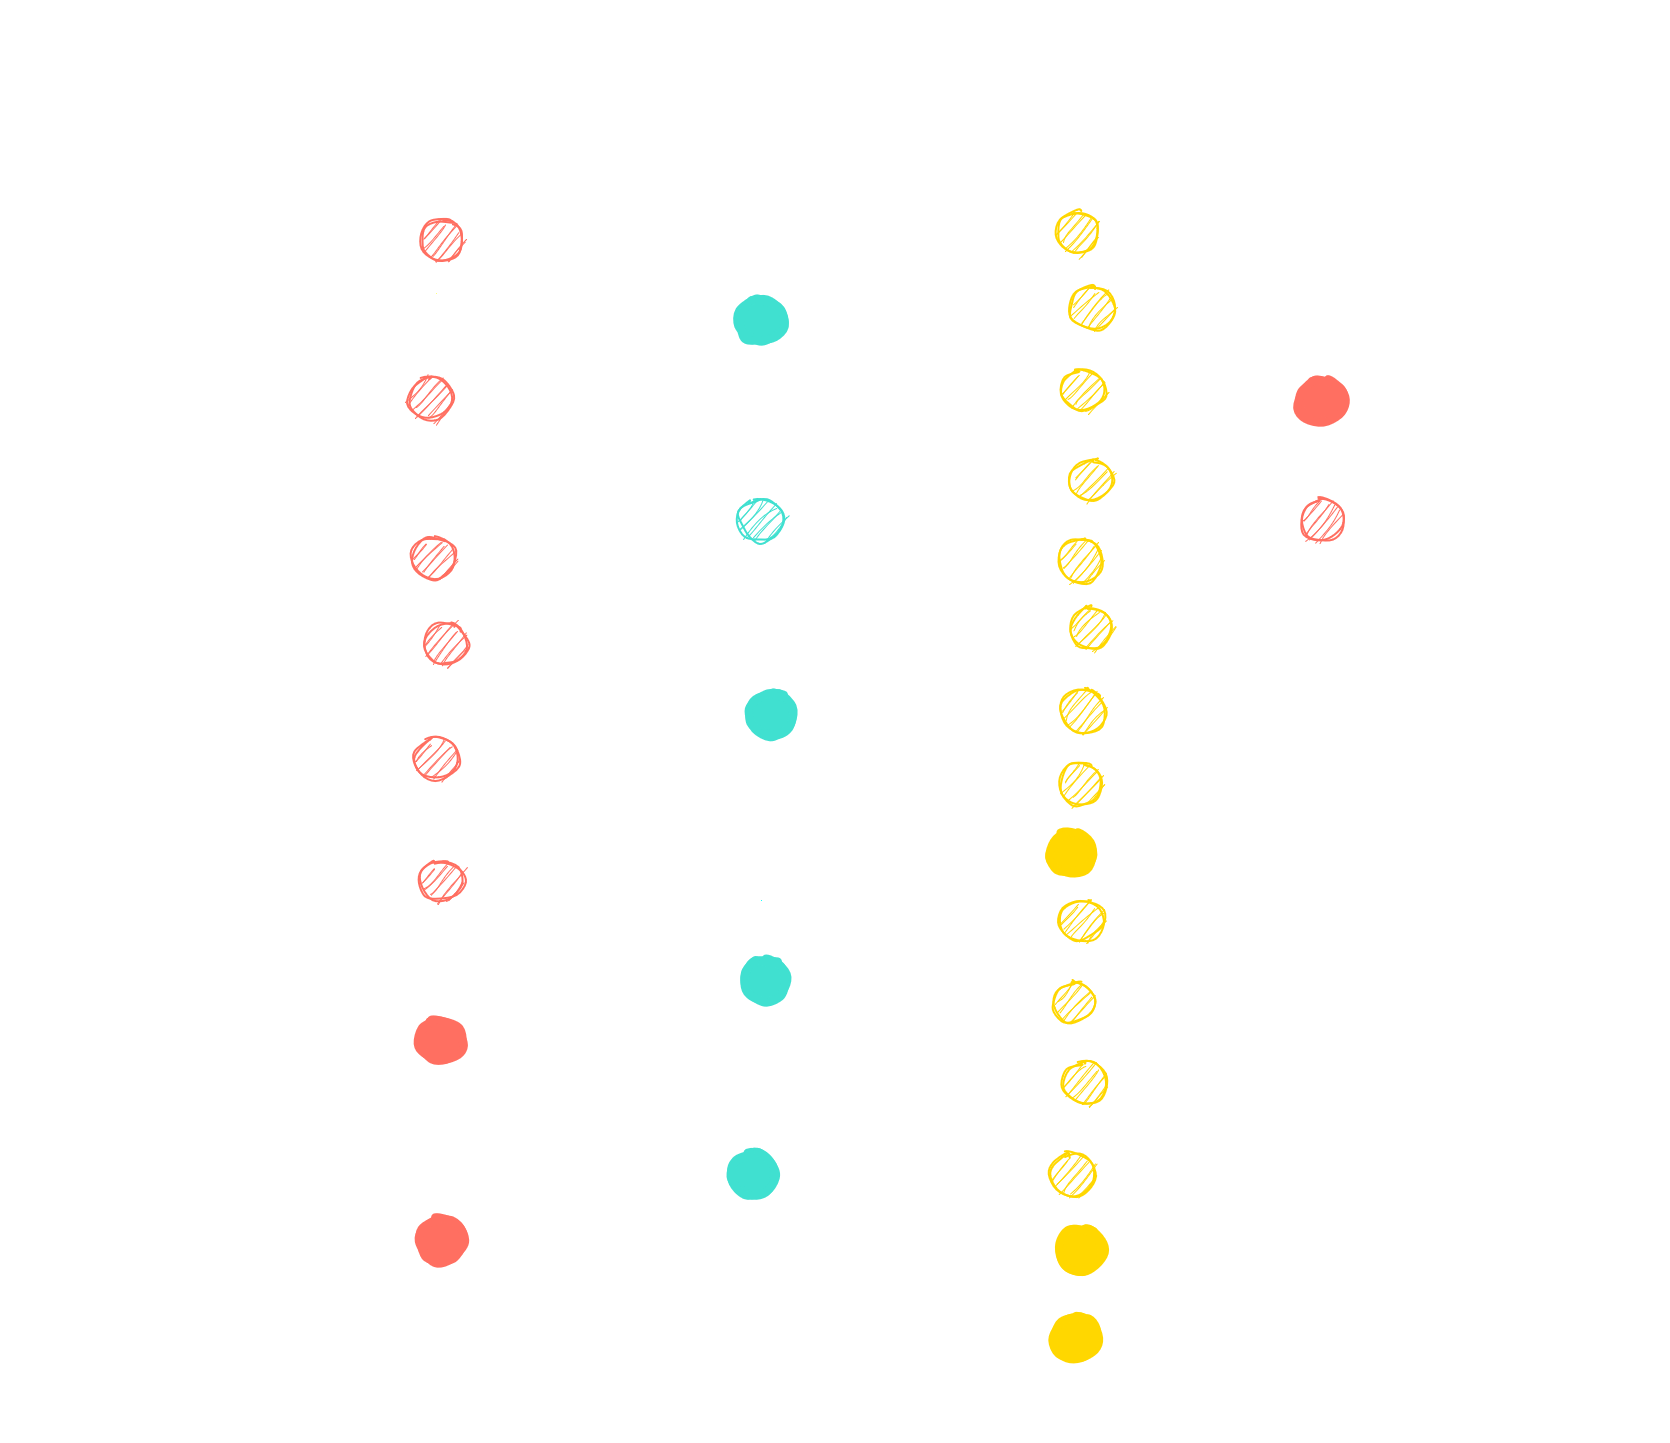
\includegraphics[scale=.13]{resources/rt2-0.png}

\end{frame}

\begin{frame}
\frametitle{Example: Amino-Mainline Bridge}

\hspace{2cm}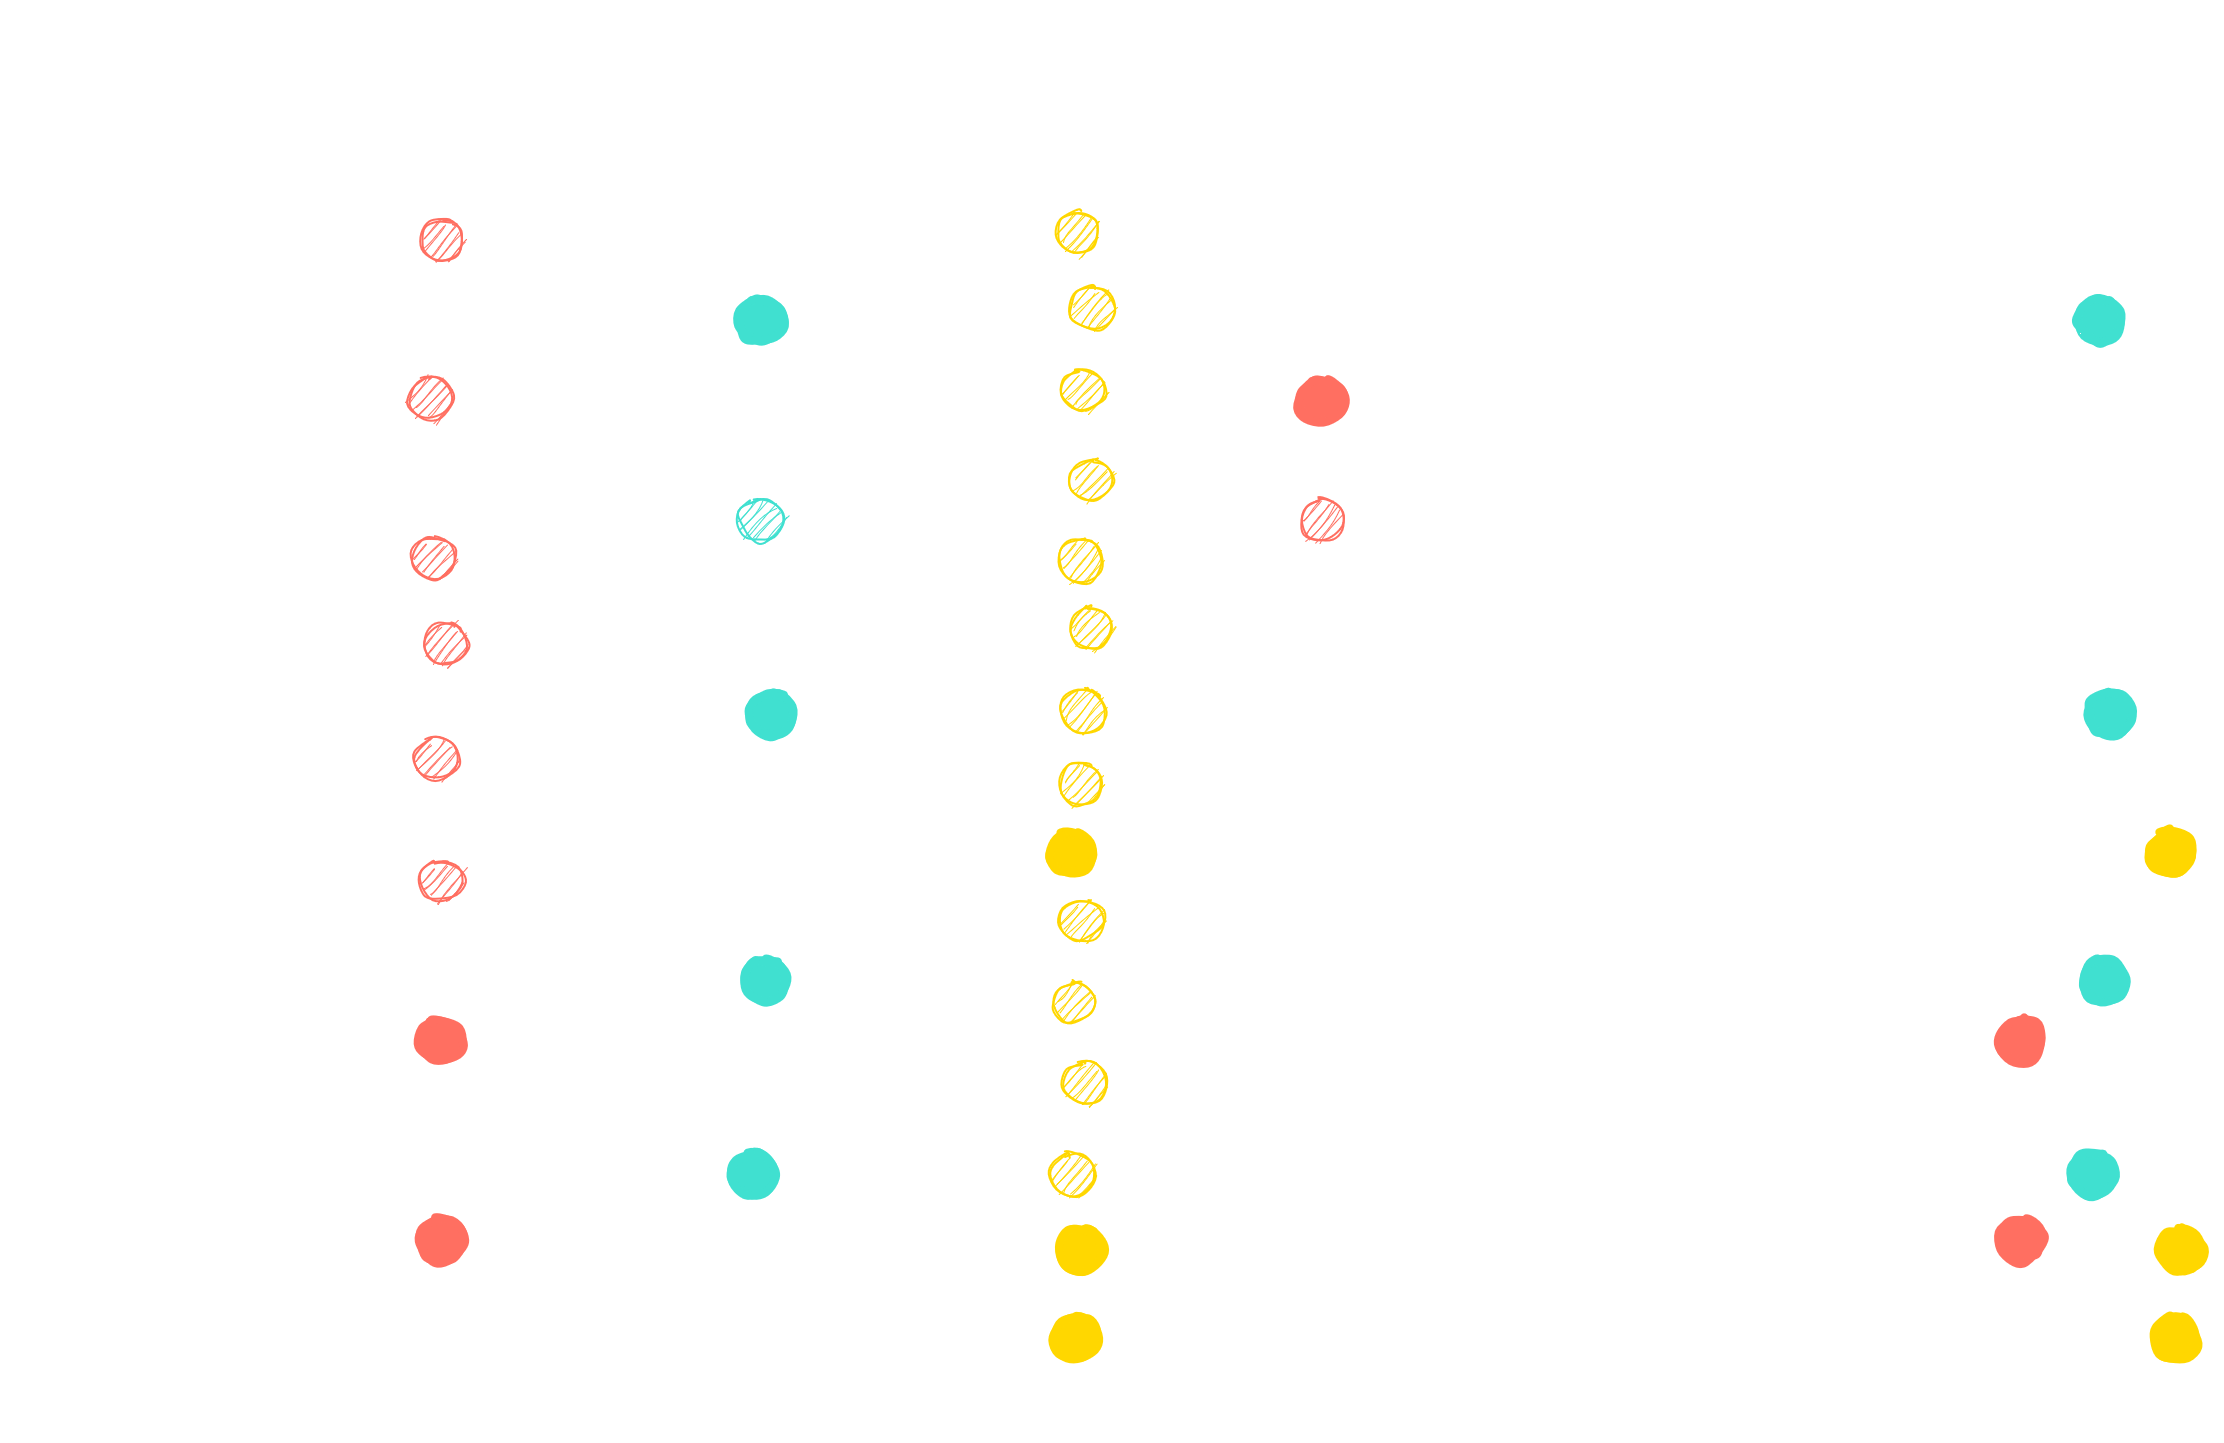
\includegraphics[scale=.13]{resources/rt2-1.png}


\end{frame}

\begin{frame}
\frametitle{Example: Amino-Mainline Bridge}

\hspace{2cm}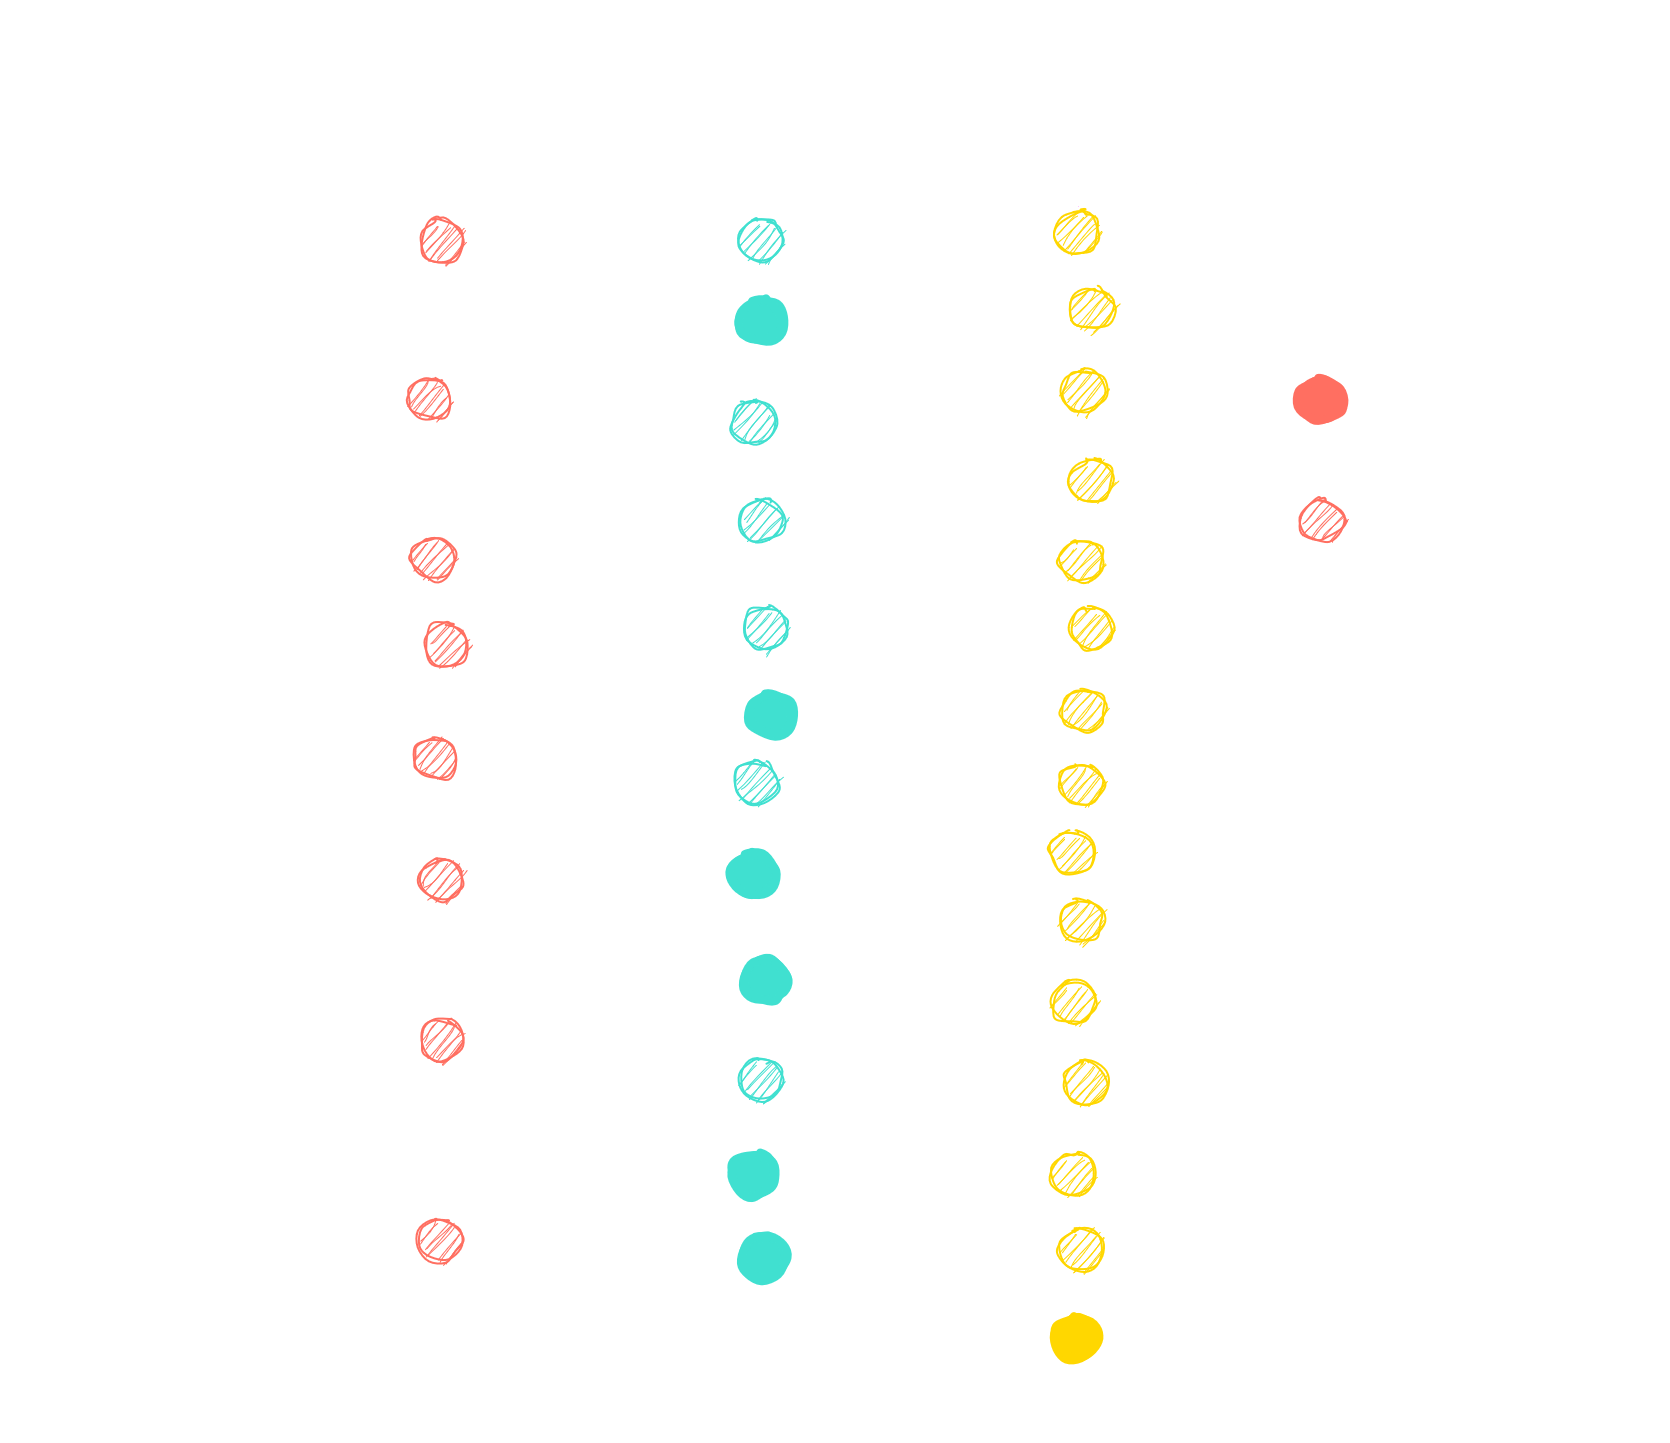
\includegraphics[scale=.13]{resources/rt3-0.png}


\end{frame}

\begin{frame}
\frametitle{Example: Amino-Mainline Bridge}

\hspace{2cm}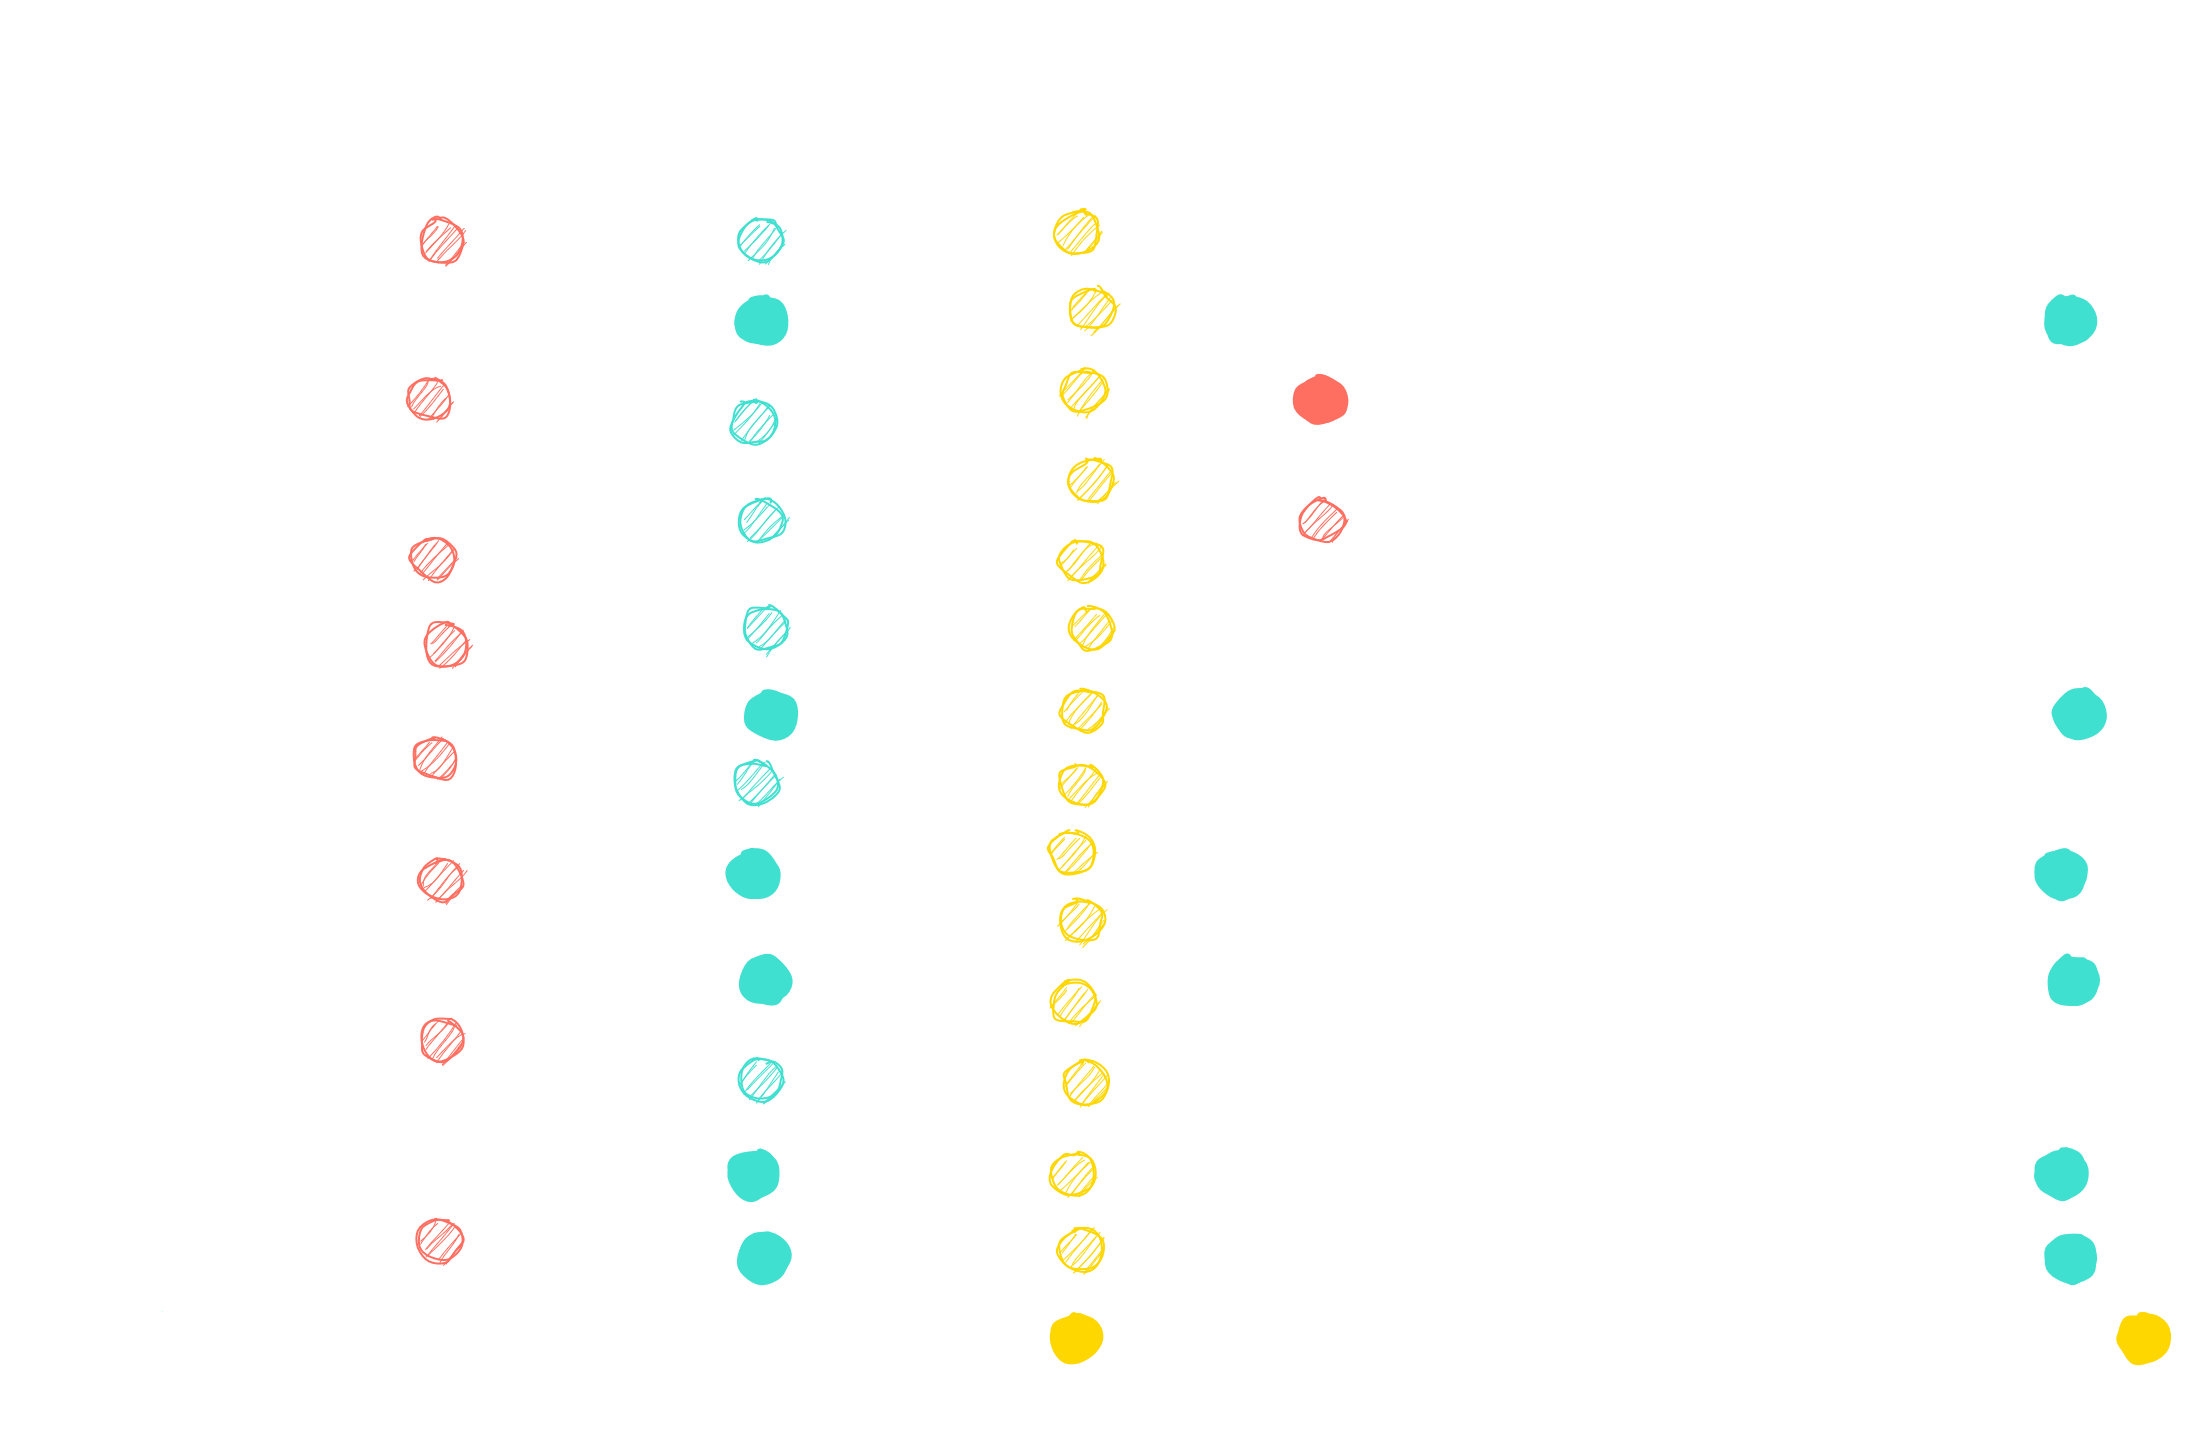
\includegraphics[scale=.13]{resources/rt3-1.png}


\end{frame}


\begin{frame}
\frametitle{Scaling}

\begin{itemize}
	\itemc Scaling is great!
	\itemc Routing table size $\approx$ routing table size for largest network \smiley
	\begin{itemize}
		\item[\greencube] Larger overhead when networks are disjoint (small set of peers participating in both networks)
	\end{itemize}
	\itemc Can be applied for much more than 2 DHT networks \smiley
\end{itemize}
\end{frame}

\begin{frame}
\frametitle{Omnidex: use cases}

\begin{itemize}
	\itemc Participation in multiple networks, or features (Provider Records, IPNS, etc.)
	\itemc Protocol evolution (e.g DHT Reader Privacy Upgrade, S/Kademlia, etc.)
	\itemc Transport compatibility
\end{itemize}
\end{frame}

\begin{frame}
\frametitle{Protocol Evolution}
\end{frame}

\begin{frame}
\frametitle{Protocol Evolution}

\hspace{2cm}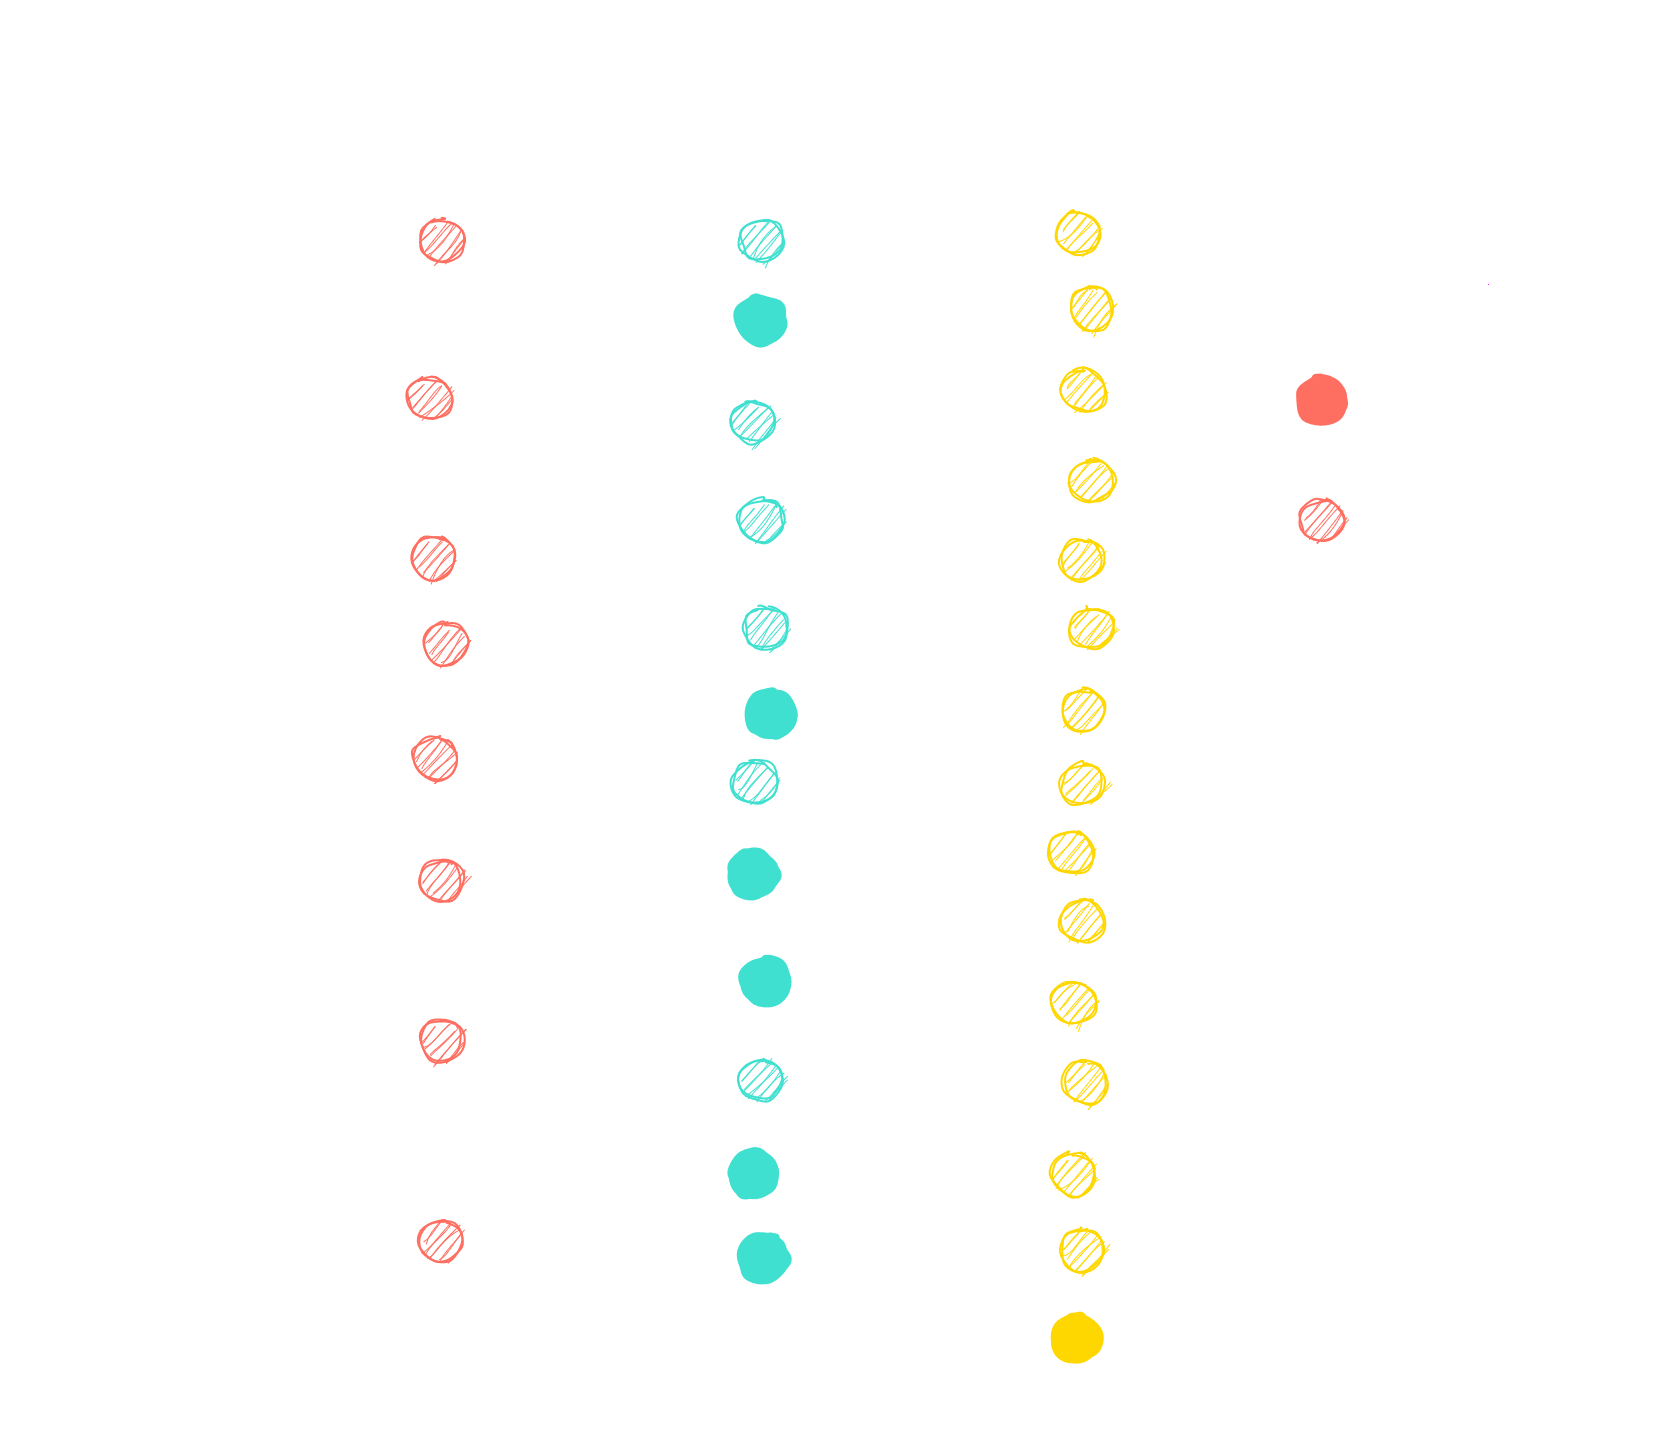
\includegraphics[scale=.13]{resources/rt4-0.png}

\end{frame}

\begin{frame}
\frametitle{Transport compatibility}

\begin{columns}[onlytextwidth]
\begin{column}{0.38\textwidth}
\begin{itemize}
	\itemc Some transports are more popular than others.
	\itemc Peers using unpopular transports may not be able to reach the closest peers.
	\itemc Browser nodes are victim of this problem in the Amino DHT
	\itemc \texttt{IPv4} vs \texttt{IPv6}
\end{itemize}
\end{column}
\begin{column}{0.58\textwidth}
    \begin{center}
    		\textbf{Amino DHT Transport Distribution}
		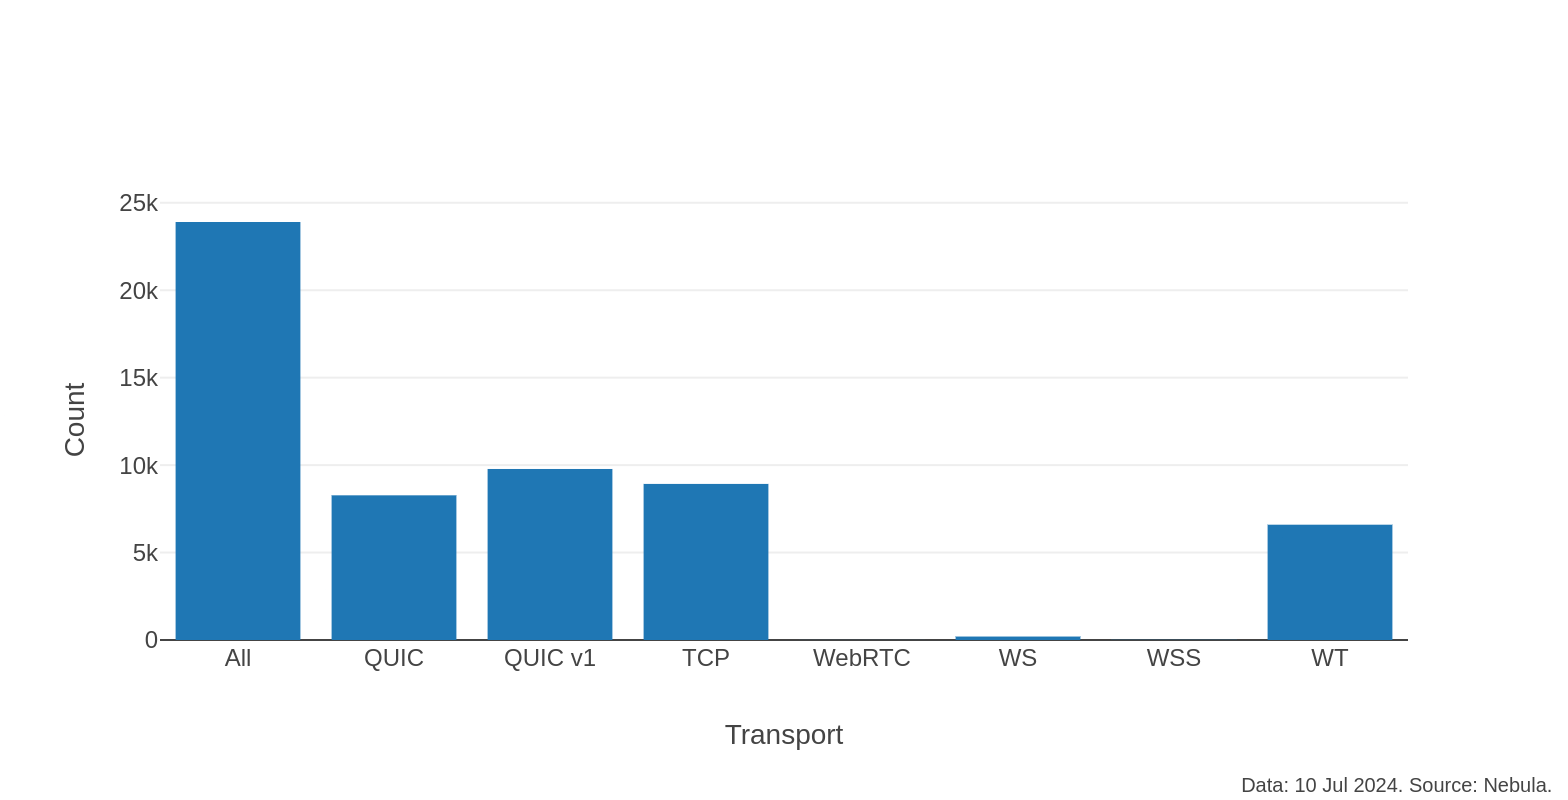
\includegraphics[width=\textwidth]{resources/dht-transport-distribution.png}
		{\small Source: \url{https://probelab.io}}
    \end{center}
\end{column}
\end{columns}
\end{frame}


\begin{frame}
\frametitle{Transport compatibility}

\hspace{1.2cm}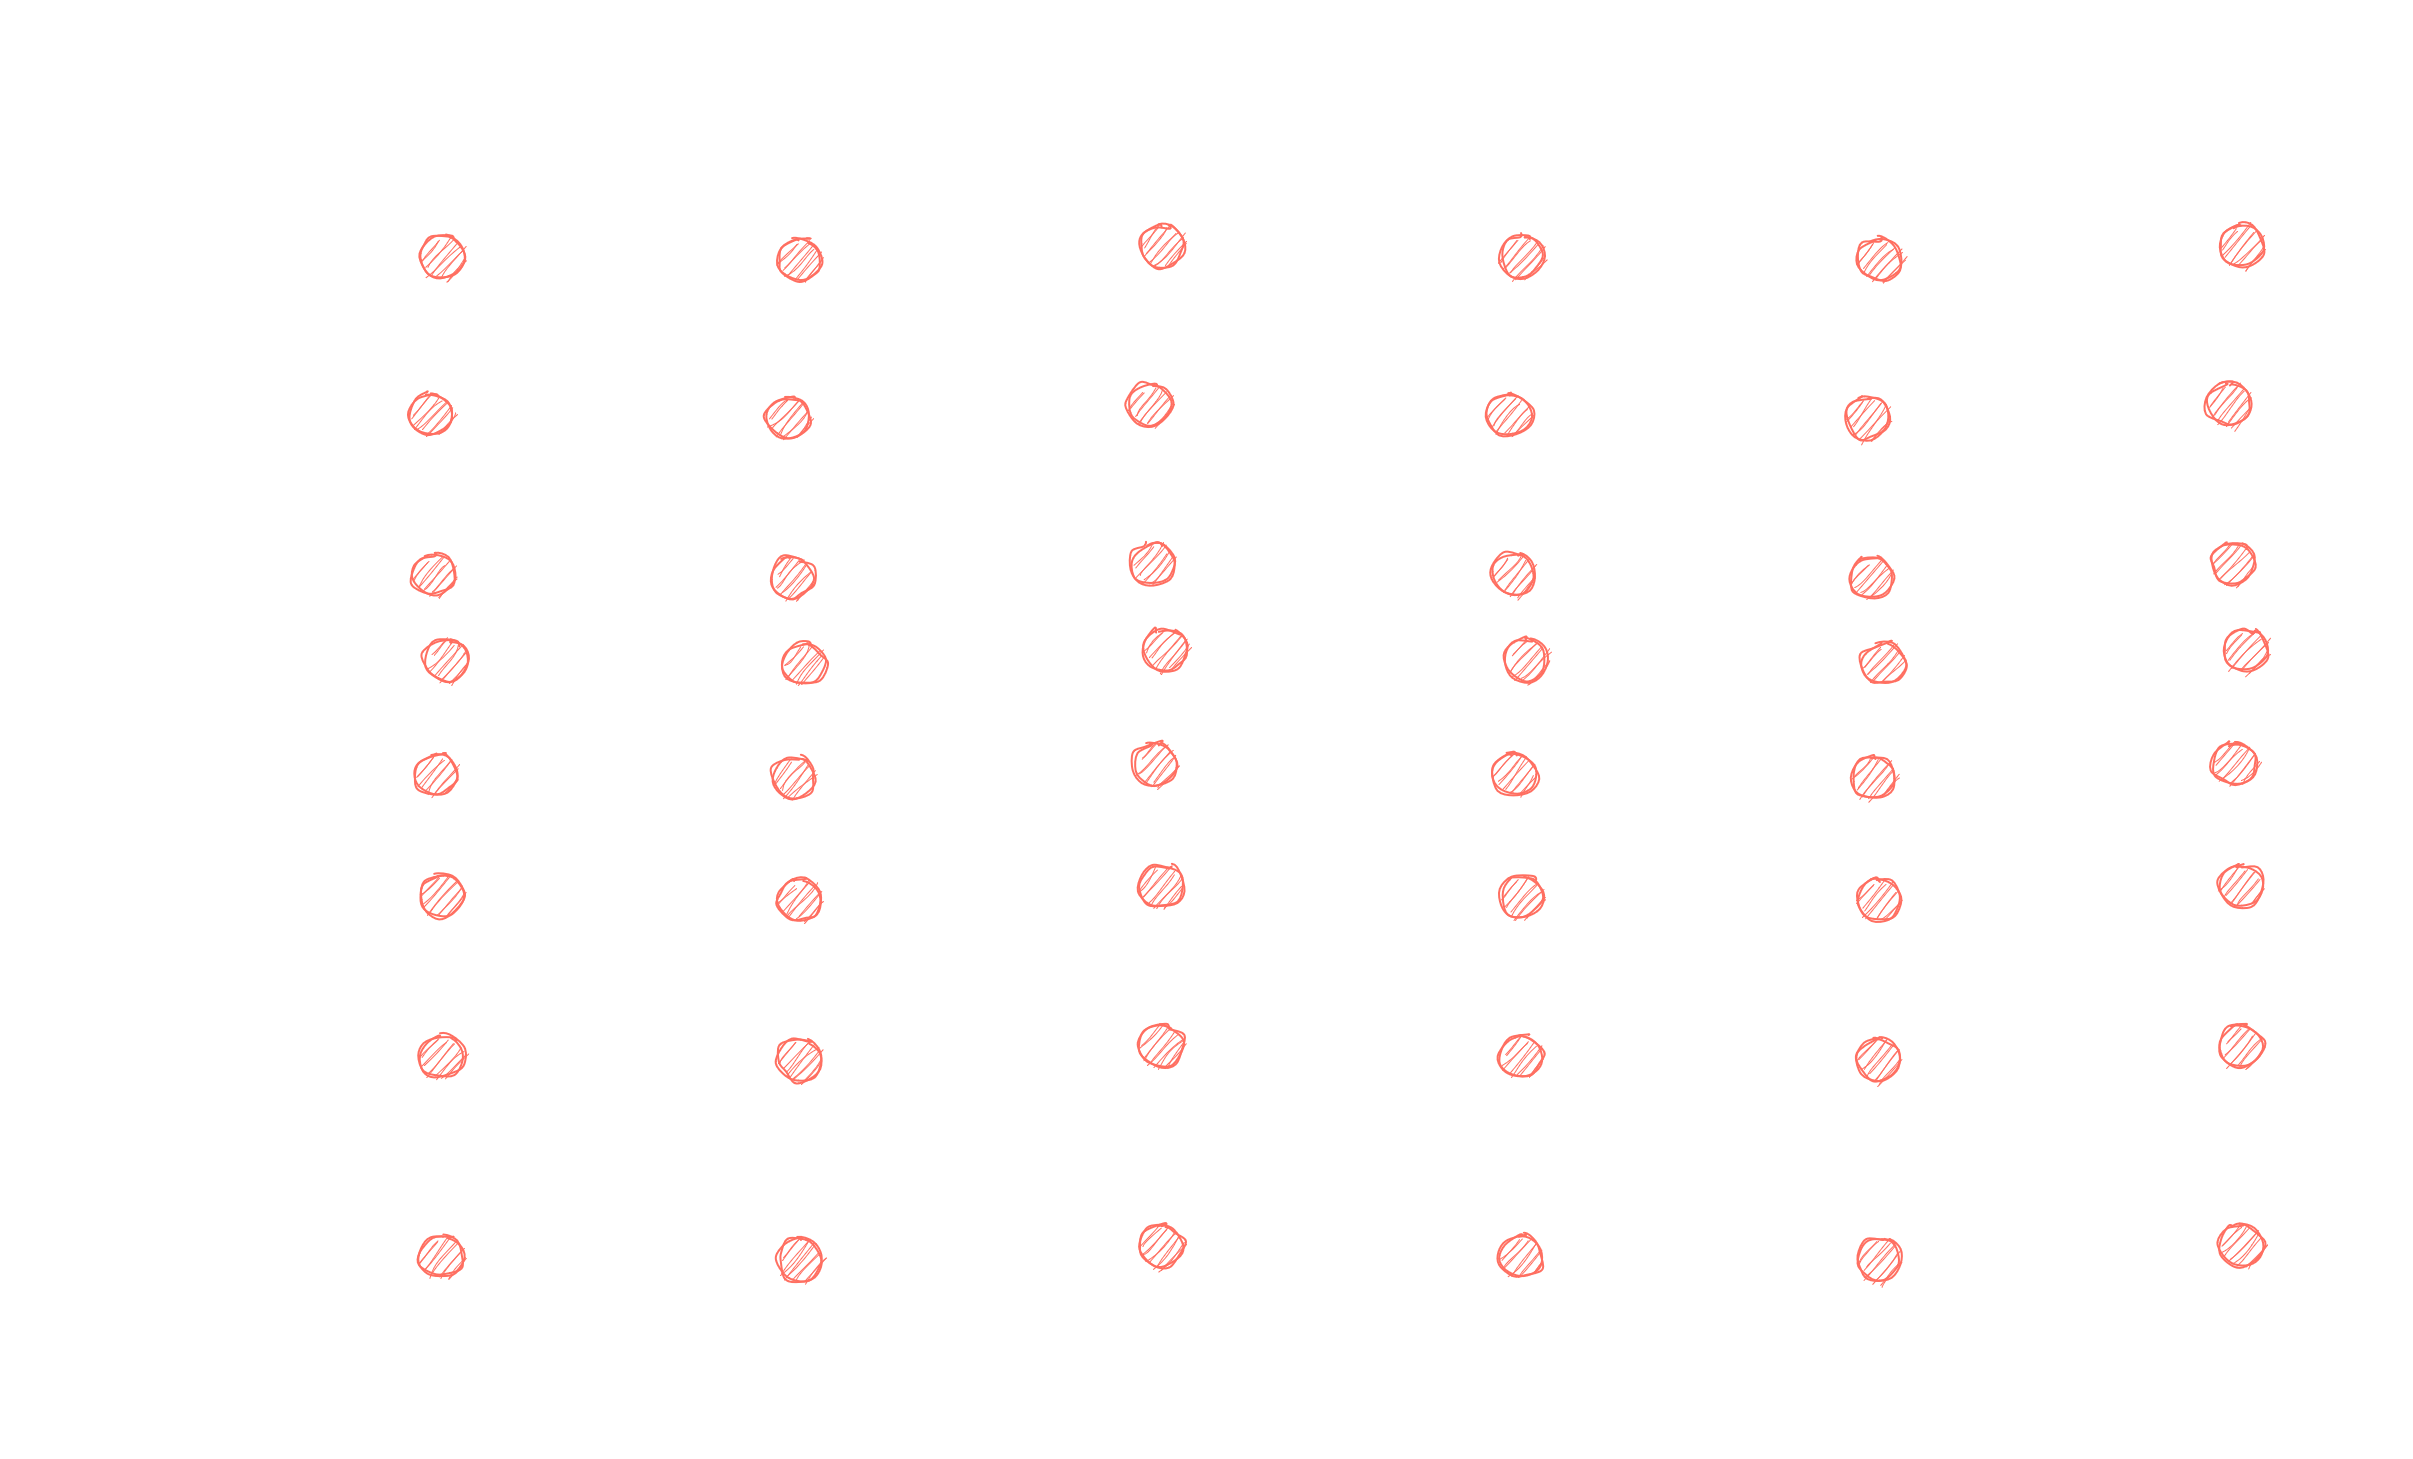
\includegraphics[scale=.13]{resources/rt5-0.png}
\end{frame}

\begin{frame}
\frametitle{Transport compatibility}

All combinations of \texttt{ip4}, \texttt{ip6}, \texttt{quic}, \texttt{webrtc}

\begin{columns}[onlytextwidth]
\begin{column}{0.38\textwidth}
\begin{itemize}
	\itemc \texttt{/ip4/quic}
	\itemc \texttt{/ip4/webrtc}
	\itemc \texttt{/ip6/quic}
	\itemc \texttt{/ip6/webrtc}
	\itemc \texttt{/ip4/quic}, \texttt{/ip4/webrtc}
	\itemc \texttt{/ip6/quic}, \texttt{/ip6/webrtc}
	\itemc \texttt{/ip4/quic}, \texttt{/ip6/webrtc}
	\itemc \texttt{/ip6/quic}, \texttt{/ip4/webrtc}
\end{itemize}
\end{column}
\begin{column}{0.58\textwidth}
\begin{itemize}
	\itemc \texttt{/ip4/quic}, \texttt{/ip6/quic}
	\itemc \texttt{/ip4/webrtc}, \texttt{/ip6/webrtc}
	\itemc \texttt{/ip4/quic}, \texttt{/ip4/webrtc}, \texttt{/ip6/quic}
	\itemc \texttt{/ip4/quic}, \texttt{/ip6/webrtc}, \texttt{/ip6/webrtc}
	\itemc \texttt{/ip4/quic}, \texttt{/ip6/quic}, \texttt{/ip6/webrtc}
	\itemc \texttt{/ip4/webrtc}, \texttt{/ip6/quic}, \texttt{/ip6/webrtc}
	\itemc \texttt{/ip4/quic}, \texttt{/ip4/webrtc}, \texttt{/ip6/quic}, \texttt{/ip6/webrtc}
\end{itemize}
\end{column}
\end{columns}
\end{frame}

\begin{frame}
\frametitle{Transport compatibility}

\begin{itemize}
	\itemc A node must be able to find the closest nodes given a specific transport
	\itemc Each transport has its own sub-DHT
	\itemc Nodes try to read \& write in all sub-DHTs they participate in
	\begin{itemize}
		\item[\greencube] This process can be optimized!
	\end{itemize}
\end{itemize}
\end{frame}

\begin{frame}
\frametitle{DHT Features}

Each node must advertise all its transport capabilities and features.

\medskip

E.g a node using transports \texttt{quic} \& \texttt{webrtc} with \texttt{ip4} \& \texttt{ip6}, participating in \texttt{IPNS} \& \texttt{provs} must advertise the following:
\medskip
\begin{itemize}
	\itemc \texttt{/ip4/quic/ipns}
	\itemc \texttt{/ip4/quic/provs}
	\itemc \texttt{/ip4/webrtc/ipns}
	\itemc \texttt{/ip4/webrtc/provs}
	\itemc \texttt{/ip6/quic/ipns}
	\itemc \texttt{/ip6/quic/provs}
	\itemc \texttt{/ip6/webrtc/ipns}
	\itemc \texttt{/ip6/webrtc/provs}
\end{itemize}
\end{frame}


\begin{frame}
\frametitle{Multi query}

\begin{itemize}
	\itemc New RPC: \texttt{FIND\_NODE\_WITH\_FEATS(key, []features)}
	\itemc Response must contain the \texttt{K} closest peers for each feature, along with supported features
	\begin{itemize}
		\item[\greencube] Overlap is expected to be high
	\end{itemize}
	\itemc Records stored \texttt{K} times in each sub-DHT
\end{itemize}
\medskip

Example: IPFS Provider Records
\begin{itemize}
	\itemc A provider will store provider records in all of its transports sub-DHTs
	\itemc Any retriever supporting common transport can find the provider record
	\itemc Because provider and retriever share at least 1 transport, retriever can open a connection to provider
\end{itemize}
\medskip
Trickier with mutable records.
\end{frame}

\begin{frame}
\frametitle{Records consistency}

\begin{enumerate}
	\itemc Records are replicated on \texttt{K} nodes in each sub-DHT
	\itemc Multiple writers of mutable records with different transports cause consistency issues
	\itemc Record holders may not receive the same set of updates
	\itemc Sync between nodes using different transports
\end{enumerate}
\end{frame}


\begin{frame}
\frametitle{Sub-DHT requirements}

Required RPCs:
\begin{itemize}
	\itemc \texttt{FIND\_NODE}, ideally \texttt{FIND\_NODE\_WITH\_FEATS}
	\itemc \texttt{READ}
	\itemc \texttt{WRITE}
\end{itemize}

\medskip

Notes:
\begin{itemize}
	\itemc Transports and features should be decoupled from one another to allow more granularity.
	\itemc Each sub-DHT can have its own requirements
	\begin{itemize}
		\item[\greencube] Secure identity (e.g S/Kademlia)
		\item[\greencube] Permissioned networks
	\end{itemize}
\end{itemize}

\end{frame}

\begin{frame}
\frametitle{\textit{Global} DHT Layers}

\begin{itemize}
	\itemc Optional participation
	\itemc Global relay \& DCUtR nodes
	\itemc \texttt{FIND\_FEATURE} to allow bootstrapping new networks from existing ones
	\itemc Global \texttt{FIND\_NODE} for increased security
\end{itemize}
\end{frame}



\begin{frame}
\frametitle{Towards standardization}

\begin{itemize}
	\itemc Transport
	\itemc Identity
	\itemc RPCs
\end{itemize}

\end{frame}

\begin{frame}
\frametitle{Going forward}

\begin{itemize}
	\itemc A first network should implement and deploy this concept
	\itemc Ideally in the libp2p codebases
	\itemc Other networks can then reuse the code to benefit from the interoperability
	\itemc When multiple networks use the same implementation, interop is trivial
	\itemc Bridges to other (non-libp2p) networks can be built after the initial implementation (e.g bittorrent mainline, ethereum discovery, etc.)
\end{itemize}
\end{frame}

\begin{frame}
\frametitle{Conclusion}

Omnidex enables:
\begin{itemize}
	\itemc Efficient use of multiple DHT networks
	\itemc Transport compatibility
	\itemc DHT protocol evolution
	\itemc Increased security
	\itemc Granular participation to DHT base layers (e.g relays)
\end{itemize}
\end{frame}


\begin{frame}
\frametitle{Q\&A}

\begin{columns}[onlytextwidth]
	\begin{column}{0.69\textwidth}
	\begin{columns}[onlytextwidth]
	\begin{column}{.2\textwidth}
		\tikz\node [circle, minimum width = \linewidth,
			path picture = {
      			\node [] at (path picture bounding box.center) {
        				
\includegraphics[width=\linewidth]{../resources/avatar.jpg}
        			};
    		}] {};
	\end{column}
	\begin{column}{.78\textwidth}
		{\Large Gui Michel (@guissou)}
	\end{column}
	\end{columns}
	\vspace{1cm}
	\begin{itemize}
		\itemc email: \texttt{guillaume@ipshipyard.com}
	\end{itemize}

	\end{column}
	\begin{column}{0.29\textwidth}
		\begin{center}
			\qrcode[height=3cm]{https://foregoing-plantain-cf9.notion.site/OmniDex-Composable-DHT-59674d72b0fe43b9a144188cedf7353c}\\
			\smallskip
			\textit{Composable DHT: Omnidex}\\
			{\small Last updated: August 2023}
		\end{center}
	\end{column}
\end{columns}

\end{frame}

\end{document}

\begin{frame}
\frametitle{Multi query}

\end{frame}

\begin{frame}
\frametitle{Multi routing table}

\end{frame}

